\documentclass[12pt, a4paper]{article}
\usepackage[margin=0.75in,footskip=0.25in]{geometry}

% Pakiety do obsługi języka polskiego i kodowania
\usepackage[T1]{fontenc}
\usepackage[polish]{babel}
\usepackage[utf8]{inputenc}
\usepackage{hyperref}

% Pakiet do zaawansowanych środowisk matematycznych
\usepackage{amsmath}

% DODANO: Pakiet do wstawiania wykresów i rysunków
\usepackage{graphicx}
\usepackage{booktabs}
\usepackage{float} % Przydatne do wymuszania pozycji [H]

\begin{document}

\begin{center}
    {\Large \textbf{Klasyfikacja i regresja dla danych tabelarycznych}}\\[0.5em]
    \textbf{Data:} \today\\
    \textbf{Autorzy:} Mateusz Stawicki, Maciej Kondratowicz
\end{center}

\tableofcontents
\newpage

\section{Klasyfikacja}

\subsection{Streszczenie}

Raport przedstawia proces budowy i ewaluacji modeli uczenia maszynowego służących do klasyfikacji kierunku wzrostu twarzoczaszki na podstawie 26 cech oraz 446 pomiarów ortodontycznych. W ramach prac przetestowano trzy głowne algorytmy: Drzewo Decyzyjne, Random Forest oraz K-Nearest Neighbors, stosując techniki nadpróbkowania (SMOTE), optymalizację hiperparametrów (Grid Search, Randomized Search) oraz zaawansowaną inżynierię cech.

\subsection{Wstępna analiza i preprocesing danych}

W pierwszej fazie prac przeprowadzono szczegółową analizę eksploracyjną zbioru danych ortodontycznych. Zbiór składa się z 446 obserwacji oraz 27 zmiennych. Zmienne objaśniające (26 cech) stanowią numeryczne pomiary twarzoczaszki pacjentów, zarejestrowane w dwóch okresach rozwoju: w 9. i 12. roku życia (są to m.in. kąty SN/MP, Facial axis, Y-axis, SNB, SNA, ANB czy stosunek AFH:PFH). Zmienną celu jest kategoryczna cecha określająca kierunek wzrostu (\textit{growth direction}) zawierająca 3 klasy: horizontal, normal, vertical.

\subsubsection{Kompletność danych i rozkład zmiennej celu}

Weryfikacja kompletności zbioru (na podstawie analizy wartości \textit{Null}) wykazała całkowity brak braków w danych dla każdej z 27 kolumn. W związku z tym, na etapie preprocesingu nie było konieczności stosowania żadnych technik uzupełniania danych.

Analiza rozkładu klas dla zmiennej docelowej \textit{growth direction} ujawniła znaczne zjawisko niezrównoważenia klas. Wystąpienia poszczególnych klas prezentują się następująco:
\begin{itemize}
    \item \textbf{normal} - 246 obserwacji,
    \item \textbf{horizontal} - 184 obserwacje,
    \item \textbf{vertical} - zaledwie 16 obserwacji.
\end{itemize}
Zdecydowana niedoreprezentacja klasy \textit{vertical} (stanowiącej niecałe 4\% całego zbioru) jest kluczowym wyzwaniem w modelowaniu i może wymagać w późniejszych etapach zastosowania odpowiednich technik balansowania klas, takich jak oversampling (np. SMOTE) lub manipulacja wagami klas w wybranych algorytmach klasyfikacyjnych.

\subsubsection{Analiza wartości odstających (Outlierów)}

Do identyfikacji wartości odstających dla zmiennych numerycznych wykorzystano metodę rozstępu międzykwartylowego (IQR -- \textit{Interquartile Range}). Zidentyfikowano łącznie 85 wystąpień wartości wykraczających poza wyznaczone dolne i górne granice (wąsy pudełkowe) w poszczególnych cechach. 

Najwięcej anomalii zaobserwowano m.in. dla kąta \texttt{12\_Mn Base angle} (8 obserwacji), \texttt{12\_SNPog} (7 obserwacji) oraz \texttt{12\_SNB} (7 obserwacji). Dwie cechy -- \texttt{9\_ANB} oraz \texttt{12\_AFH:PFH} - nie wykazały żadnych wartości odstających według przyjętego kryterium. Z uwagi na biomedyczny charakter zbioru danych, zidentyfikowane wartości najprawdopodobniej odzwierciedlają naturalną, rzadszą zmienność anatomiczną pacjentów i silne wady zgryzu, w związku z czym nie zdecydowano się na ich usunięcie.

\begin{figure}[H]
    \centering % Wyśrodkowanie obrazka
    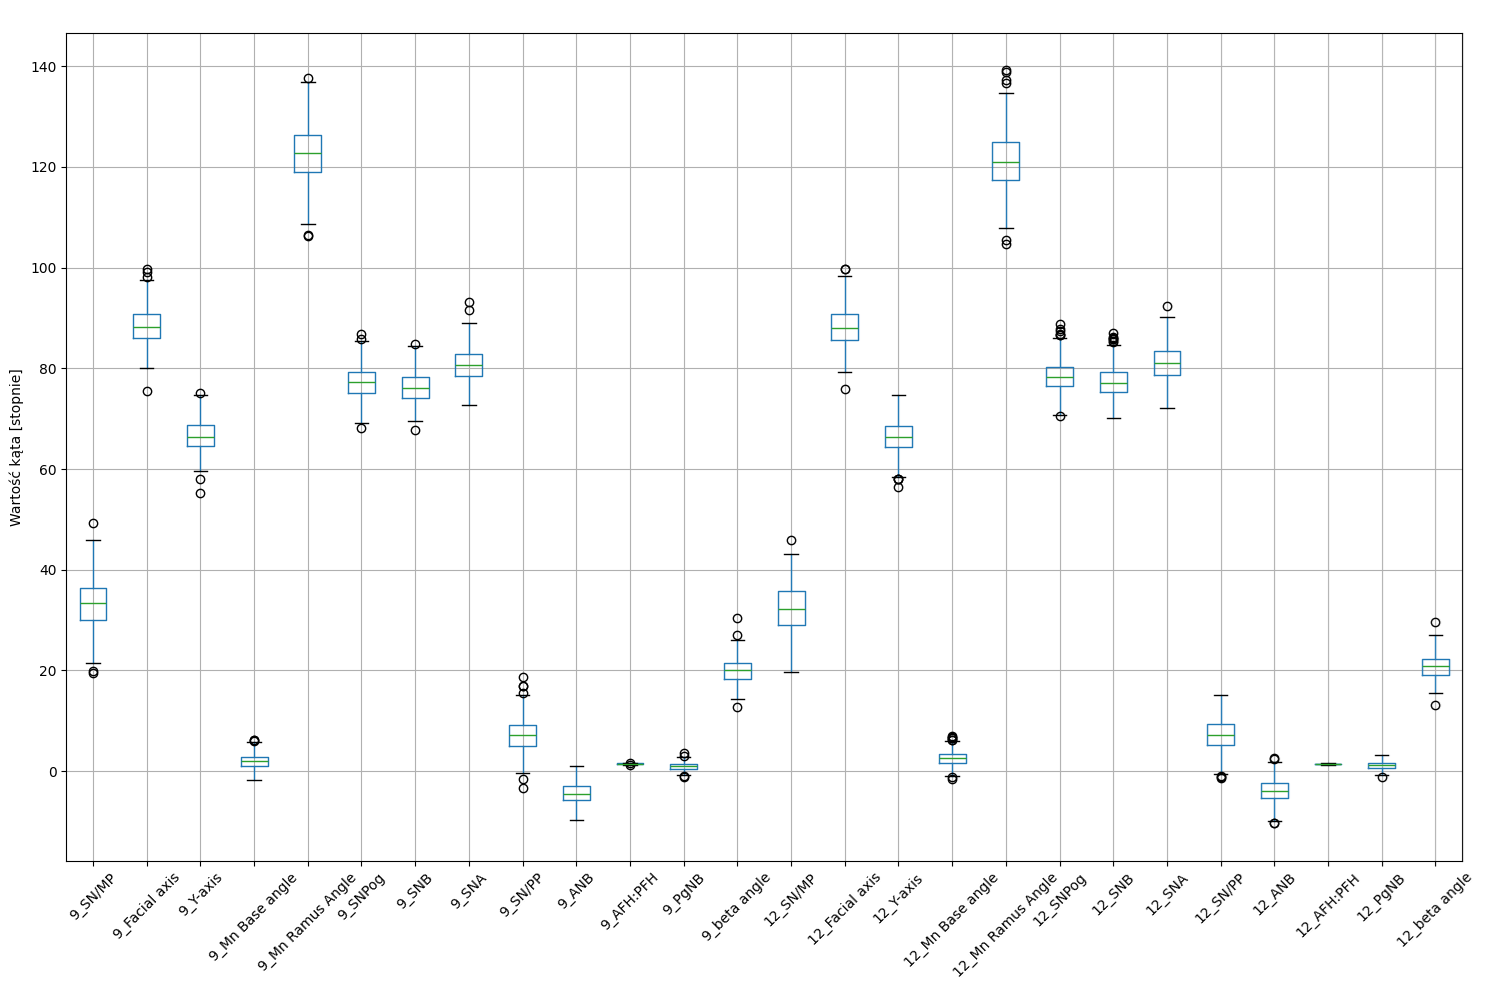
\includegraphics[width=0.9\textwidth]{outliers.png}
    \caption{Wizualizacja wartości odstających} % To doda numer i opis
    \label{fig:outliers} % Etykieta do odwoływania się w tekście
\end{figure}

\subsubsection{Analiza korelacji}

W celu zbadania zależności liniowych między 26 zmiennymi objaśniającymi, wygenerowano macierz korelacji z zastosowaniem klastrowania hierarchicznego (Rysunek \ref{fig:correlations}). Analiza wykresu ujawnia powszechne występowanie silnego zjawiska współliniowości.

Najbardziej zauważalną zależnością jest bardzo wysoka, dodatnia korelacja pomiędzy pomiarami tej samej cechy zarejestrowanymi w 9. i 12. roku życia. Wartości współczynnika korelacji dla tych par nierzadko przekraczają próg 0.8 (co jest szczególnie widoczne m.in. dla zmiennych \texttt{12\_SNA} i \texttt{9\_SNA}, a także \texttt{SN/MP}, \texttt{SNB} czy \texttt{Mn Ramus Angle}). Wskazuje to na istotny fakt anatomiczny: u większości pacjentów proporcje szkieletowe pozostają relatywnie stabilne w czasie rozwoju.

Ponadto widoczne są grupy cech silnie powiązanych w tym samym wieku pomiaru. Wiele z tych cech jest ze sobą powiązanych anatomicznie, co naturalnie prowadzi do powstawania silnych korelacji dodatnich i ujemnych. Przykładowo, zmienne takie jak \texttt{SN/MP}, \texttt{AFH:PFH}, \texttt{Facial axis} oraz \texttt{Y-axis} tworzą wyraźny blok o wysokiej korelacji dodatniej.

Występowanie tak licznych i silnych korelacji (wielowspółliniowość) wymaga zachowania szczególnej ostrożności podczas selekcji cech do modelu. Włączenie silnie skorelowanych zmiennych przeważnie nie wnosi dodatkowej mocy predykcyjnej. Stanowi to silną przesłankę do rozważenia zastosowania metod redukcji wymiarowości.

\begin{figure}[H]
    \centering
    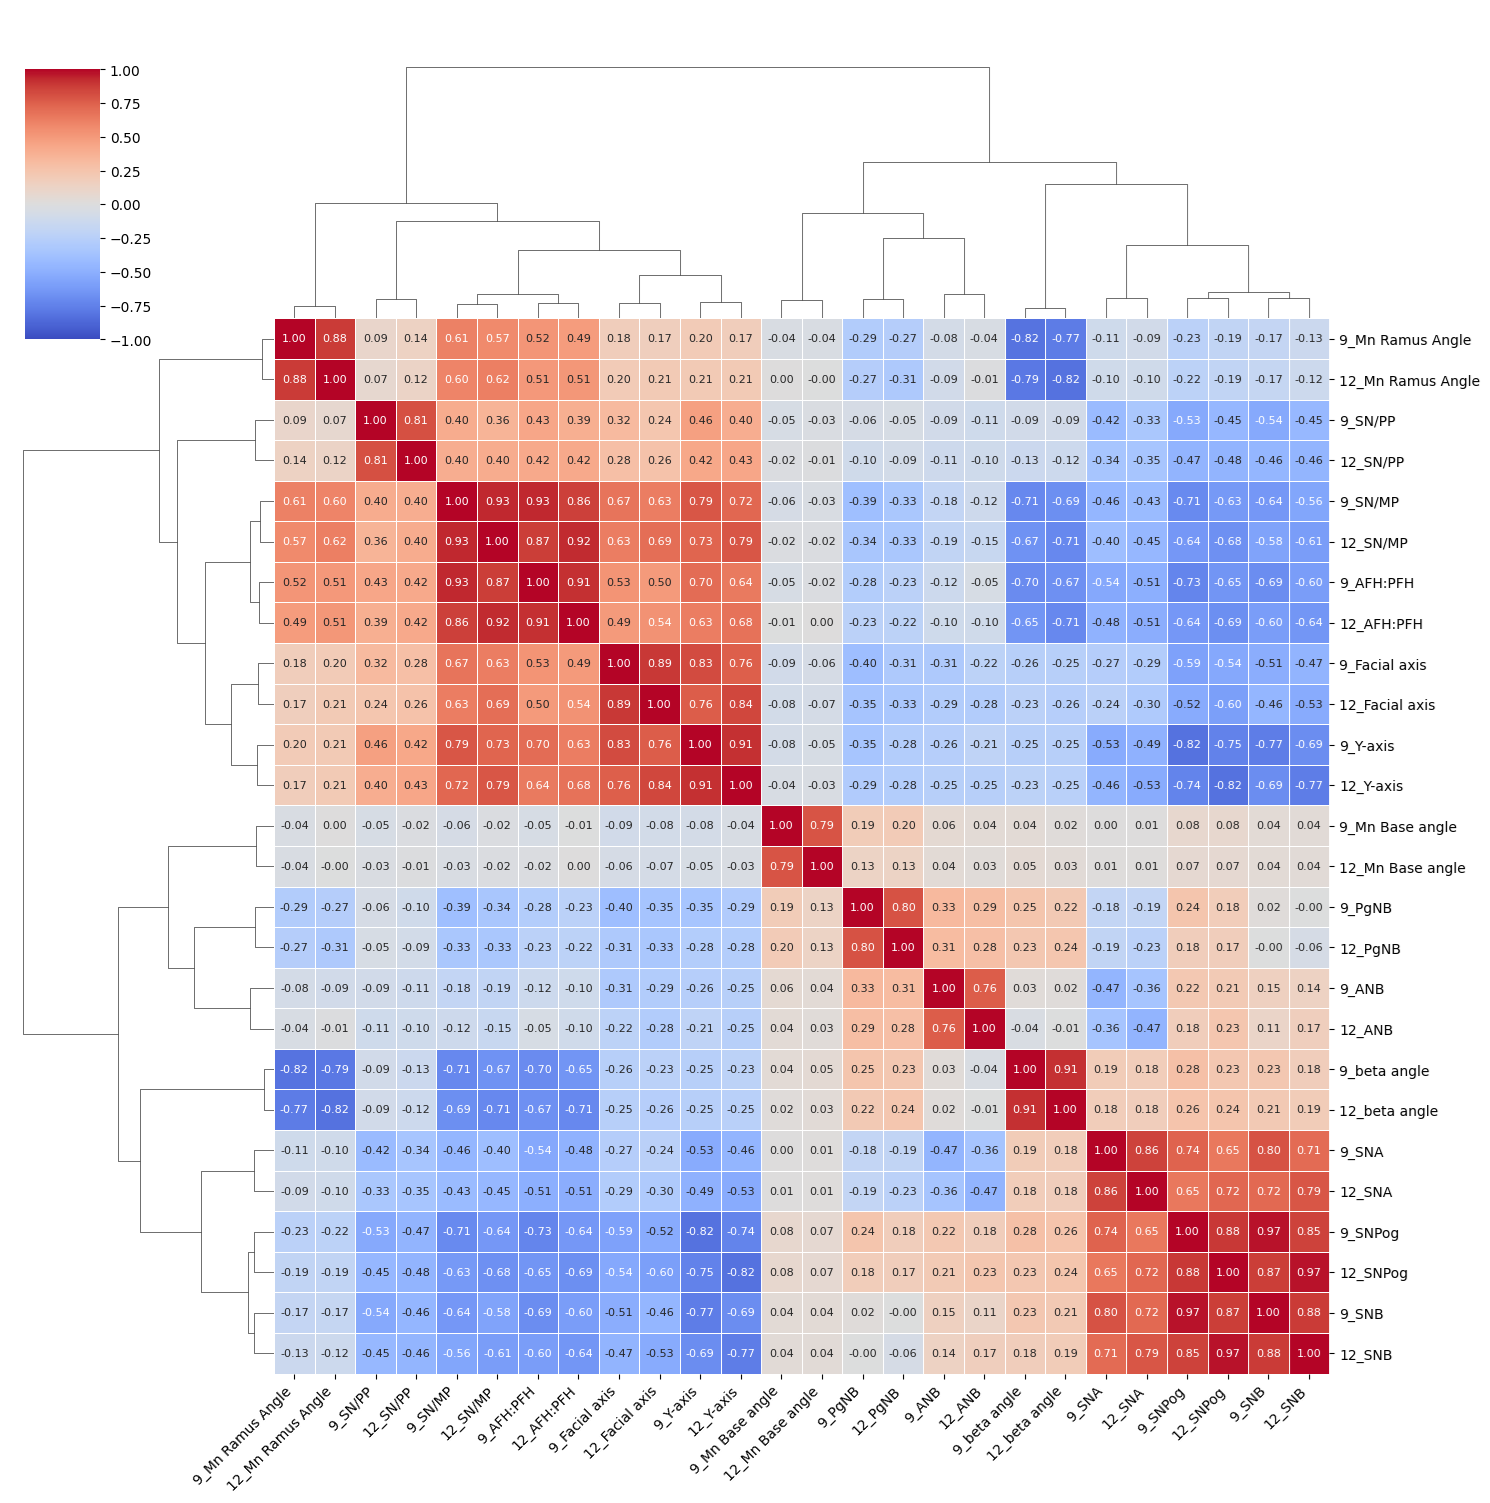
\includegraphics[width=1\textwidth]{corelations.png}
    \caption{Macierz korelacji zmiennych}
    \label{fig:correlations}
\end{figure}

\subsubsection{Standaryzacja danych}

Z uwagi na fakt, że cechy opierają się na miarach kątowych i proporcjach o różnych zakresach i wariancjach, algorytmy podatne na skalę mogłyby faworyzować zmienne o większych wartościach bezwzględnych. 

Aby temu zapobiec, przed algorytmem K-Nearest Neighbors, zbiór poddano procesowi standaryzacji (skalowania). Cechy zostały przekształcone w taki sposób, aby ich wartość oczekiwana (średnia) wynosiła 0, a odchylenie standardowe 1. W celu uniknięcia wycieku informacji, skaler został dopasowany wyłącznie na zbiorze treningowym, a następnie wykorzystany do transformacji zarówno zbioru uczącego, jak i testowego.






\subsection{Kroswalidacja}
W celu rzetelnej oceny algorytmów uczenia maszynowego oraz optymalizacji ich hiperparametrów, zastosowano zaawansowany schemat walidacji krzyżowej. Ze względu na losowość procesów uczenia, eksperymenty należy powtarzać, dlatego zdecydowano się na wykorzystanie powtórzonej walidacji krzyżowej. Skonfigurowano podział zbioru na 5 podzbiorów, a cały proces powtarzano 3-krotnie. Taka parametryzacja skutkuje przeprowadzeniem 15 niezależnych iteracji ucząco-testujących dla każdego ewaluowanego modelu. Pozwala to na to, aby wyniki zostały opisane statystycznie z wykorzystaniem miar takich jak średnia i odchylenie standardowe. Takie podejście znacząco zwiększa wiarygodność ewaluacji i pozwala na rzetelną ocenę siły modelu. Kluczowym aspektem wybranego schematu jest jego warstwowość. Zbiór danych charakteryzuje się silnym niezrównoważeniem klas, co jest szczególnie widoczne na przykładzie klasy \textit{vertical}, która liczy zaledwie 16 obserwacji. Zwykły losowy podział mógłby doprowadzić do sytuacji, w której ta mniejszościowa klasa w ogóle nie znalazłaby się w zbiorze testowym lub treningowym w danej iteracji. Mechanizm warstwowy rozwiązuje ten problem, gwarantując zachowanie oryginalnych proporcji klas we wszystkich wygenerowanych podzbiorach.

\subsection{Drzewo Decyzyjne}

\subsubsection{Bazowe Drzewo Decyzyjne}

Celem tego eksperymentu było stworzenie i ocena bazowego modelu drzewa decyzyjnego.

W procesie kroswalidacji model uzyskał średni wynik F1-macro na poziomie $0{,}5268 \pm 0{,}0812$. Szczegółowe wyniki klasyfikacji na zbiorze testowym przedstawiono w Tabeli \ref{tab:dt_baseline_results}.

\begin{table}[h!]
\centering
\caption{Metryki klasyfikacji dla bazowego modelu Drzewa Decyzyjnego}
\label{tab:dt_baseline_results}
\begin{tabular}{@{}lcccc@{}}
\toprule
\textbf{Klasa} & \textbf{Precision} & \textbf{Recall} & \textbf{F1-score} & \textbf{Support} \\ \midrule
0              & 0,71               & 0,73            & 0,72              & 37               \\
1              & 0,76               & 0,74            & 0,75              & 50               \\
2              & 0,33               & 0,33            & 0,33              & 3                \\ \midrule
\textbf{Accuracy}       & \multicolumn{2}{c}{---}       & \textbf{0,72}     & 90               \\
\textbf{Macro avg}      & 0,60               & 0,60            & 0,60              & 90               \\
\textbf{Weighted avg}   & 0,72               & 0,72            & 0,72              & 90               \\ \bottomrule
\end{tabular}
\end{table}

Ponadto, na Rysunku \ref{fig:cm_dt_baseline} przedstawiono macierz pomyłek, która obrazuje trudności modelu w poprawnej klasyfikacji mniejszościowej klasy 2.

\begin{figure}[H]
    \centering
    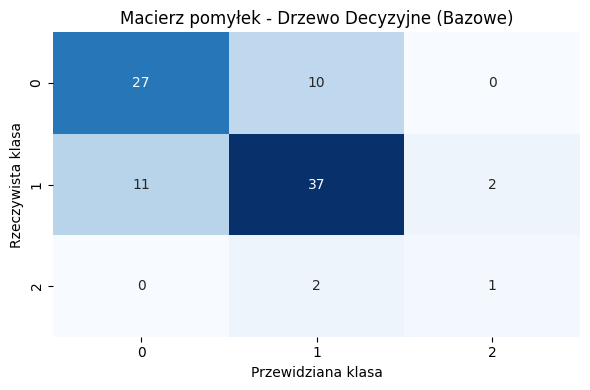
\includegraphics[width=0.6\textwidth]{confusion_matrix_dt.png} 
    \caption{Macierz pomyłek dla bazowego modelu Drzewa Decyzyjnego}
    \label{fig:cm_dt_baseline}
\end{figure}


\subsubsection{Drzewo Decyzyjne z techniką SMOTE}

W kolejnym etapie eksperymentu sprawdzono wpływ techniki \textit{oversamplingu} SMOTE na zdolność modelu do rozpoznawania klasy mniejszościowej (Klasa 2). Średni wynik F1-macro uzyskany w kroswalidacji wzrósł do $0{,}5908 \pm 0{,}1233$, jednak szczegółowa analiza na zbiorze testowym (Tabela \ref{tab:dt_smote_results}) ujawniła istotne problemy modelu.

\begin{table}[H]
\centering
\caption{Metryki klasyfikacji dla modelu Drzewa Decyzyjnego po zastosowaniu SMOTE}
\label{tab:dt_smote_results}
\begin{tabular}{@{}lcccc@{}}
\toprule
\textbf{Klasa} & \textbf{Precision} & \textbf{Recall} & \textbf{F1-score} & \textbf{Support} \\ \midrule
0              & 0,70               & 0,76            & 0,73              & 37               \\
1              & 0,76               & 0,74            & 0,75              & 50               \\
2              & 0,00               & 0,00            & 0,00              & 3                \\ \midrule
\textbf{Accuracy}       & \multicolumn{2}{c}{---}       & \textbf{0,72}     & 90               \\
\textbf{Macro avg}      & 0,49               & 0,50            & 0,49              & 90               \\
\textbf{Weighted avg}   & 0,71               & 0,72            & 0,71              & 90               \\ \bottomrule
\end{tabular}
\end{table}

\begin{figure}[H]
    \centering
    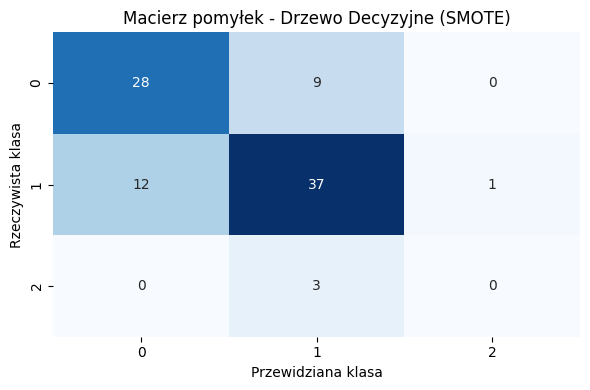
\includegraphics[width=0.7\textwidth]{cm_dt_smote.png}
    \caption{Macierz pomyłek dla modelu z SMOTE. Widoczny całkowity brak poprawnych klasyfikacji dla klasy 2.}
    \label{fig:cm_dt_smote}
\end{figure}

Zastosowanie SMOTE wpłynęło negatywnie na stabilność modelu w odniesieniu do zbioru testowego. Choć wynik kroswalidacji sugerował poprawę, ostateczny wynik F1-score dla klasy 2 spadł do 0,00. Przyczyną tego stanu rzeczy jest prawdopodobnie zbyt mała liczność klasy mniejszościowej. 

Algorytm SMOTE generuje syntetyczne próbki na podstawie k-najbliższych sąsiadów; przy ekstremalnie małej liczbie punktów, nowo utworzone dane mogą drastycznie odbiegać od rzeczywistego rozkładu, prowadząc do silnego \textit{overfittingu} (przeuczenia) do szumu. W rezultacie model bazowy z poprzedniego etapu, mimo braku balansowania, radził sobie lepiej z ogólną generalizacją (F1-macro = 0,60) niż model wspomagany SMOTE (F1-macro = 0,49).


\subsubsection{Optymalizacja Drzewa Decyzyjnego (Grid Search + SMOTE)}

Kolejnym etapem pracy z pojedynczym drzewem decyzyjnym była próba optymalizacji hiperparametrów przy jednoczesnym zastosowaniu techniki SMOTE. Wykorzystano procedurę \textit{Grid Search}. 

W wyniku przeszukiwania przestrzeni parametrów wyłoniono optymalny model charakteryzujący się następującymi cechami:
\begin{itemize}
    \item \textbf{Criterion:} entropy,
    \item \textbf{Max depth:} 5,
    \item \textbf{Min samples leaf:} 1,
    \item \textbf{Min samples split:} 2.
\end{itemize}

Model ten uzyskał najwyższy dotychczasowy średni wynik F1-macro w kroswalidacji wynoszący $0{,}6233 \pm 0{,}1004$. Szczegółowe metryki dla zbioru testowego zaprezentowano w Tabeli \ref{tab:dt_opt_results}.

\begin{table}[H]
\centering
\caption{Metryki klasyfikacji dla zoptymalizowanego modelu Drzewa Decyzyjnego (SMOTE + Grid Search)}
\label{tab:dt_opt_results}
\begin{tabular}{@{}lcccc@{}}
\toprule
\textbf{Klasa} & \textbf{Precision} & \textbf{Recall} & \textbf{F1-score} & \textbf{Support} \\ \midrule
0              & 0,87               & 0,70            & 0,78              & 37               \\
1              & 0,78               & 0,92            & 0,84              & 50               \\
2              & 1,00               & 0,33            & 0,50              & 3                \\ \midrule
\textbf{Accuracy}       & \multicolumn{2}{c}{---}       & \textbf{0,81}     & 90               \\
\textbf{Macro avg}      & 0,88               & 0,65            & 0,71              & 90               \\
\textbf{Weighted avg}   & 0,82               & 0,81            & 0,80              & 90               \\ \bottomrule
\end{tabular}
\end{table}

\begin{figure}[H]
    \centering
    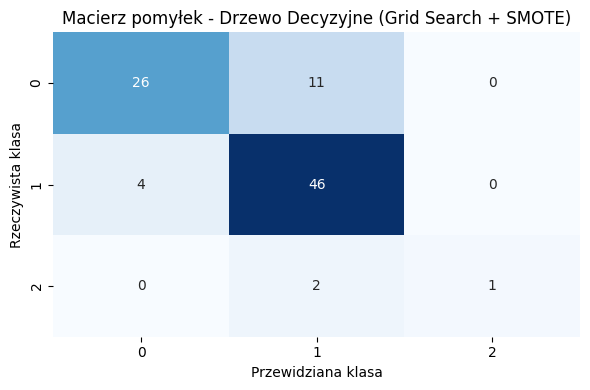
\includegraphics[width=0.7\textwidth]{cm_dt_opt.png}
    \caption{Macierz pomyłek dla zoptymalizowanego modelu. Widoczna poprawa w detekcji klasy 2.}
    \label{fig:cm_dt_opt}
\end{figure}

Wprowadzenie optymalizacji hiperparametrów pozwoliło na skuteczne wykorzystanie potencjału techniki SMOTE. Kluczowe okazało się ograniczenie głębokości drzewa (\texttt{max\_depth: 5}), co zapobiegło obserwowanemu wcześniej przeuczeniu do syntetycznych próbek. 

Model po raz pierwszy poprawnie zidentyfikował obiekt z mniejszościowej klasy 2 (\textit{Recall} = 0,33), utrzymując przy tym bardzo wysoką precyzję (1,00). Ogólna dokładność (\textit{Accuracy}) wzrosła z $0{,}72$ do $0{,}81$, a miara F1-macro na zbiorze testowym osiągnęła poziom $0{,}71$, co stanowi istotny progres względem modelu bazowego ($0{,}60$) oraz modelu SMOTE bez optymalizacji ($0{,}49$).


\subsubsection*{Inżynieria cech i zaawansowana optymalizacja (Engineering + SMOTE + GridSearch)}

Ostatnim etapem pracy z pojedynczym drzewem decyzyjnym było zastosowanie inżynierii cech. Przeprowadzono następujące operacje:
\begin{itemize}
    \item \textbf{Inżynieria cech:} Utworzono zmienne typu \textit{Delta}, obliczając różnicę w pomiarach między 12. a 9. rokiem życia dla każdego parametru.
    \item \textbf{Selekcja cech:} Usunięto surowe dane z 9. roku życia (zawarte w delcie i pomiarach z 12. roku) oraz wyeliminowano zmienne o korelacji wyższej niż $0,9$ w celu redukcji wielowspółliniowości. Zredukowano liczbę cech do 23.
    \item \textbf{Modelowanie:} Zastosowano \textit{ImbPipeline} łączący SMOTE z drzewem o zbalansowanych wagach klas (\textit{class\_weight='balanced'}).
\end{itemize}

Najlepsze parametry wyłonione przez \textit{Grid Search}: \texttt{criterion: gini, max\_depth: 3, min\_samples\_leaf: 2, min\_samples\_split: 10}. Wyniki przedstawiono w Tabeli \ref{tab:dt_eng_results}.

\begin{table}[H]
\centering
\caption{Metryki dla modelu z inżynierią cech i optymalizacją}
\label{tab:dt_eng_results}
\begin{tabular}{@{}lcccc@{}}
\toprule
\textbf{Klasa} & \textbf{Precision} & \textbf{Recall} & \textbf{F1-score} & \textbf{Support} \\ \midrule
0              & 0,90               & 0,70            & 0,79              & 37               \\
1              & 0,85               & 0,88            & 0,86              & 50               \\
2              & 0,33               & 1,00            & 0,50              & 3                \\ \midrule
\textbf{Accuracy}       & \multicolumn{2}{c}{---}       & \textbf{0,81}     & 90               \\
\textbf{Macro avg}      & 0,69               & 0,86            & 0,72              & 90               \\
\textbf{Weighted avg}   & 0,85               & 0,81            & 0,82              & 90               \\ \bottomrule
\end{tabular}
\end{table}

\begin{figure}[H]
    \centering
    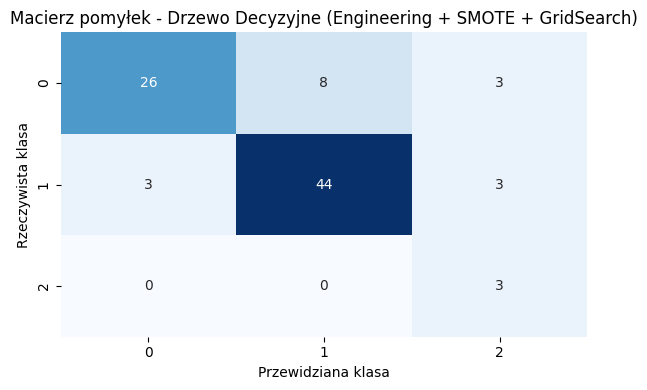
\includegraphics[width=0.7\textwidth]{cm_dt_engineered.png}
    \caption{Macierz pomyłek dla modelu z inżynierią cech. Zwraca uwagę pełna wykrywalność klasy 2.}
    \label{fig:cm_dt_eng}
\end{figure}

Wprowadzenie cech różnicowych (\textit{Delta}) oraz agresywna redukcja wymiarowości przyniosły najlepszy rezultat pod względem czułości modelu. Kluczowym osiągnięciem jest uzyskanie \textbf{Recall = 1,00 dla klasy 2}, co oznacza, że model poprawnie zidentyfikował wszystkich pacjentów z grupy mniejszościowej. 

Niska precyzja dla tej klasy ($0,33$) przy jednoczesnym wzroście ogólnego F1-macro do 0,72 sugeruje, że model stał się „liberalny” w diagnozowaniu klasy mniejszościowej (częstsze fałszywe alarmy). Bardzo płytkie drzewo (\texttt{max\_depth: 3}) zapewnia doskonałą interpretowalność i odporność na przeuczenie.



\subsection{Random Forest}

\subsubsection{Bazowy Random Forest}

Celem tego eksperymentu było przetestowanie bazowego modelu Lasu Losowego, składającego się ze 100 drzew decyzyjnych. W procesie kroswalidacji model uzyskał średni wynik F1-macro na poziomie $0{,}5602 \pm 0{,}0869$. Szczegółowa analiza metryk wykazuje istotne problemy z rozpoznawaniem klas mniejszościowych.

Szczegółowe wyniki klasyfikacji na zbiorze testowym przedstawiono w Tabeli \ref{tab:rf_baseline_results}.

\begin{table}[H]
\centering
\caption{Metryki klasyfikacji dla bazowego modelu Random Forest}
\label{tab:rf_baseline_results}
\begin{tabular}{@{}lcccc@{}}
\toprule
\textbf{Klasa} & \textbf{Precision} & \textbf{Recall} & \textbf{F1-score} & \textbf{Support} \\ \midrule
0              & 0,88               & 0,81            & 0,85              & 37               \\
1              & 0,82               & 0,92            & 0,87              & 50               \\
2              & 0,00               & 0,00            & 0,00              & 3                \\ \midrule
\textbf{Accuracy}       & \multicolumn{2}{c}{---}       & \textbf{0,84}     & 90               \\
\textbf{Macro avg}      & 0,57               & 0,58            & 0,57              & 90               \\
\textbf{Weighted avg}   & 0,82               & 0,84            & 0,83              & 90               \\ \bottomrule
\end{tabular}
\end{table}

\begin{figure}[H]
    \centering
    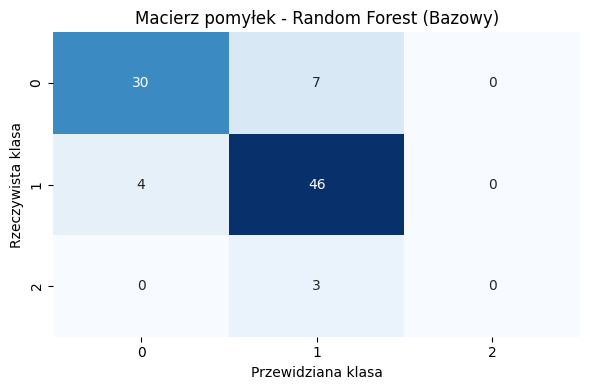
\includegraphics[width=0.7\textwidth]{rf_base.png}
    \caption{Macierz pomyłek dla modelu Random Forest}
    \label{fig:rf_base}
\end{figure}

Model Random Forest osiągnął bardzo wysoką ogólną dokładność (\textit{Accuracy} = 0,84). Bardzo dobrze radzi sobie z odróżnianiem klasy 0 (\textit{normal}) i 1 (\textit{horizontal}), uzyskując dla nich wyniki F1-score na poziomie 0,85-0,87. Podobnie jak w przypadku bazowego drzewa decyzyjnego, algorytm całkowicie zignorował klasę 2 (\textit{vertical}). Wartości precyzji i czułości dla tej klasy wynoszą 0,00.

Wyniki te wskazują na konieczność zastosowania metod balansowania klas, takich jak SMOTE lub korekta wag klas (\textit{class\_weight}), w celu poprawy zdolności predykcyjnej modelu dla rzadkich przypadków medycznych.


\subsubsection{Random Forest z techniką SMOTE}

Kolejnym etapem było sprawdzenie skuteczności lasu losowego po zastosowaniu algorytmu \textit{oversamplingu} SMOTE wewnątrz potoku przetwarzania (\textit{pipeline}). Celem było zniwelowanie negatywnego wpływu niezrównoważenia klas na zdolność modelu do detekcji rzadkich przypadków (\textit{vertical growth}).

W procesie kroswalidacji model uzyskał średni wynik F1-macro na poziomie $0{,}6594 \pm 0{,}1142$, co stanowi istotną poprawę względem wersji bazowej ($0{,}5602$). Szczegółowe metryki uzyskane na zbiorze testowym zaprezentowano w Tabeli \ref{tab:rf_smote_results}.

\begin{table}[H]
\centering
\caption{Metryki klasyfikacji dla modelu Random Forest z techniką SMOTE}
\label{tab:rf_smote_results}
\begin{tabular}{@{}lcccc@{}}
\toprule
\textbf{Klasa} & \textbf{Precision} & \textbf{Recall} & \textbf{F1-score} & \textbf{Support} \\ \midrule
0              & 0,86               & 0,84            & 0,85              & 37               \\
1              & 0,87               & 0,90            & 0,88              & 50               \\
2              & 1,00               & 0,67            & 0,80              & 3                \\ \midrule
\textbf{Accuracy}       & \multicolumn{2}{c}{---}       & \textbf{0,87}     & 90               \\
\textbf{Macro avg}      & 0,91               & 0,80            & 0,84              & 90               \\
\textbf{Weighted avg}   & 0,87               & 0,87            & 0,87              & 90               \\ \bottomrule
\end{tabular}
\end{table}

\begin{figure}[H]
    \centering
    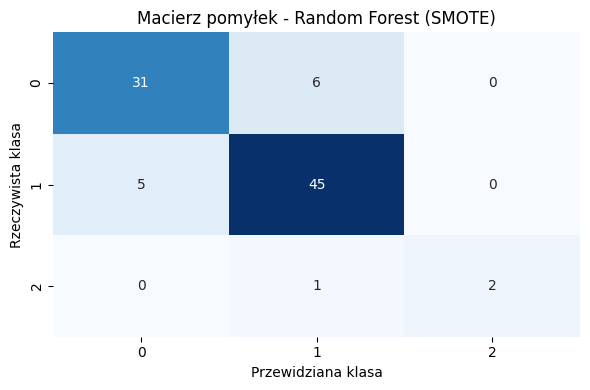
\includegraphics[width=0.7\textwidth]{rf_smote.png}
    \caption{Macierz pomyłek dla modelu Random Forest}
    \label{fig:rf_smote}
\end{figure}

Zastosowanie SMOTE pozwoliło modelowi na skuteczną identyfikację klasy 2. Uzyskanie \textit{Recall} na poziomie 0,67 (przy perfekcyjnej precyzji 1,00) oznacza, że model poprawnie rozpoznał 2 z 3 przypadków mniejszościowych, nie generując przy tym żadnych fałszywych alarmów (\textit{False Positives}) dla tej klasy. Ogólna dokładność (\textit{Accuracy}) wzrosła do poziomu 0,87, a miara F1-macro na zbiorze testowym osiągnęła bardzo wysoki wynik \textbf{0,84}. Jest to znaczący progres w stosunku do modelu bazowego (0,57). Mimo skupienia się na balansowaniu danych, model utrzymał bardzo wysoką skuteczność dla klas 0 i 1 (F1-score odpowiednio 0,85 i 0,88), co świadczy o dobrej generalizacji i braku negatywnego wpływu syntetycznych próbek na główne trendy w danych.

Model Random Forest połączony z techniką SMOTE okazał się dotychczas najbardziej zbalansowanym i skutecznym klasyfikatorem, oferującym wysoką precyzję przy jednoczesnej zdolności do wykrywania przypadków odstających anatomicznie.



\subsubsection{Optymalizacja Random Forest (Grid Search + SMOTE)}

W celu dalszej poprawy zdolności predykcyjnych oraz stabilności modelu, przeprowadzono optymalizację hiperparametrów lasu losowego przy użyciu procedury \textit{Grid Search}. Proces ten połączono z techniką balansowania SMOTE w ramach potoku przetwarzania, co pozwoliło na przeszukanie 216 kombinacji parametrów w 15 iteracjach kroswalidacji.

W wyniku optymalizacji wyłoniono model o następujących parametrach:
\begin{itemize}
    \item \textbf{n\_estimators:} 100,
    \item \textbf{max\_depth:} None (brak ograniczenia),
    \item \textbf{max\_features:} 'sqrt',
    \item \textbf{min\_samples\_leaf:} 1,
    \item \textbf{min\_samples\_split:} 10.
\end{itemize}

Zoptymalizowany model uzyskał najwyższy dotychczas średni wynik F1-macro w kroswalidacji wynoszący $0{,}6774 \pm 0{,}0999$ (poprawa względem $0{,}6594$ dla modelu SMOTE bez optymalizacji). Szczegółowe metryki dla zbioru testowego zaprezentowano w Tabeli \ref{tab:rf_opt_results}.

\begin{table}[H]
\centering
\caption{Metryki klasyfikacji dla zoptymalizowanego modelu Random Forest (Grid Search + SMOTE)}
\label{tab:rf_opt_results}
\begin{tabular}{@{}lcccc@{}}
\toprule
\textbf{Klasa} & \textbf{Precision} & \textbf{Recall} & \textbf{F1-score} & \textbf{Support} \\ \midrule
0              & 0,86               & 0,84            & 0,85              & 37               \\
1              & 0,87               & 0,90            & 0,88              & 50               \\
2              & 1,00               & 0,67            & 0,80              & 3                \\ \midrule
\textbf{Accuracy}       & \multicolumn{2}{c}{---}       & \textbf{0,87}     & 90               \\
\textbf{Macro avg}      & 0,91               & 0,80            & 0,84              & 90               \\
\textbf{Weighted avg}   & 0,87               & 0,87            & 0,87              & 90               \\ \bottomrule
\end{tabular}
\end{table}

\begin{figure}[H]
    \centering
    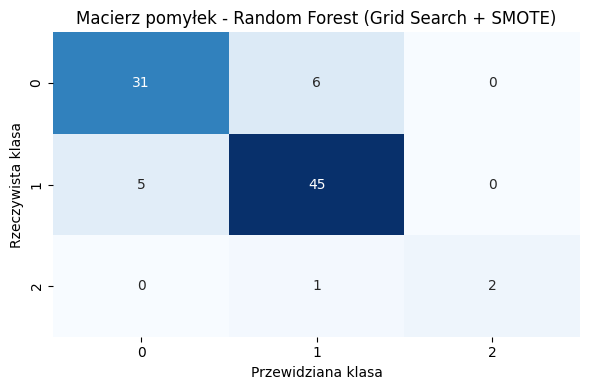
\includegraphics[width=0.7\textwidth]{rf_opt.png}
    \caption{Macierz pomyłek dla zoptymalizowanego modelu Random Forest}
    \label{fig:rf_opt}
\end{figure}

Choć wyniki na zbiorze testowym są zbliżone do modelu przed optymalizacją, wzrost średniego wyniku kroswalidacji (z 0,66 na 0,68) oraz niższe odchylenie standardowe wskazują na lepszą zdolność modelu do generalizacji na nieznanych danych. Model utrzymał bardzo wysoką precyzję dla klasy 2 (1,00), poprawnie klasyfikując 2 z 3 przypadków.



\subsubsection{Efektywna czasowo optymalizacja Random Forest (Randomized Search + SMOTE)}

Kluczowym aspektem tego eksperymentu była wydajność obliczeniowa. Podczas gdy poprzedni model optymalizowany metodą Grid Search wymagał 1 minuty i 23 sekund na znalezienie najlepszych parametrów, Randomized Search zakończył pracę w zaledwie 43 sekundy, co stanowi niemal dwukrotne przyspieszenie procesu przy zachowaniu zbliżonej jakości predykcji.

W wyniku losowania 50 kombinacji wyłoniono model o parametrach:
\begin{itemize}
    \item \textbf{n\_estimators:} 487,
    \item \textbf{max\_depth:} 40,
    \item \textbf{max\_features:} 'sqrt',
    \item \textbf{min\_samples\_leaf:} 3,
    \item \textbf{min\_samples\_split:} 3.
\end{itemize}

Średni wynik F1-macro w kroswalidacji wyniósł $0{,}6752 \pm 0{,}0954$. Szczegółowe wyniki na zbiorze testowym przedstawiono w Tabeli \ref{tab:rf_random_results}.

\begin{table}[H]
\centering
\caption{Metryki klasyfikacji dla modelu Random Forest (Randomized Search + SMOTE)}
\label{tab:rf_random_results}
\begin{tabular}{@{}lcccc@{}}
\toprule
\textbf{Klasa} & \textbf{Precision} & \textbf{Recall} & \textbf{F1-score} & \textbf{Support} \\ \midrule
0              & 0,83               & 0,81            & 0,82              & 37               \\
1              & 0,85               & 0,88            & 0,86              & 50               \\
2              & 1,00               & 0,67            & 0,80              & 3                \\ \midrule
\textbf{Accuracy}       & \multicolumn{2}{c}{---}       & \textbf{0,84}     & 90               \\
\textbf{Macro avg}      & 0,89               & 0,79            & 0,83              & 90               \\
\textbf{Weighted avg}   & 0,85               & 0,84            & 0,84              & 90               \\ \bottomrule
\end{tabular}
\end{table}

\begin{figure}[H]
    \centering
    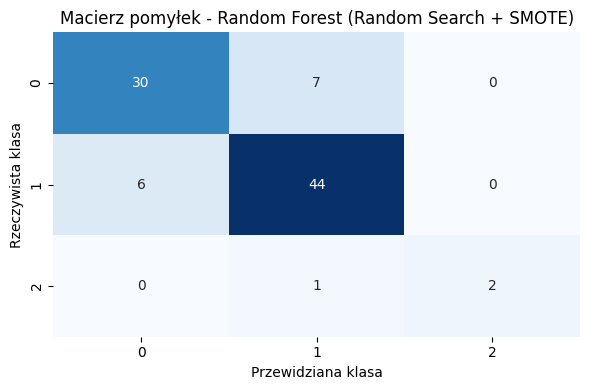
\includegraphics[width=0.7\textwidth]{rf_opt_rand.png}
    \caption{Macierz pomyłek dla Randomized Search modelu Random Forest}
    \label{fig:rf_opt_rand}
\end{figure}

Randomized Search okazał się znacznie efektywniejszy czasowo. Pozwoliło to na przetestowanie znacznie większej liczby drzew (487 zamiast 100) bez nadmiernego obciążenia zasobów. Wynik F1-macro dla klasy 2 pozostał na wysokim poziomie 0,80 (Recall 0,67). Oznacza to, że mimo szybszego procesu optymalizacji, model nie stracił zdolności do detekcji rzadkich przypadków patologicznych. Choć ogólna dokładność (\textit{Accuracy} = 0,84) jest nieznacznie niższa niż w przypadku pełnej siatki (0,87), model ten uczy się 2 razy szybciej.



\subsubsection{Zaawansowana inżynieria cech (Engineering + Ratios + SMOTE)}

Wzorując się na sukcesie inżynierii cech w bazowym drzewie decyzyjnym, zdecydowano się na wdrożenie analogicznego, lecz poszerzonego procesu dla algorytmu Random Forest. Z uwagi na powszechne w zbiorze zjawisko wielowspółliniowości, które wymaga szczególnej ostrożności podczas selekcji cech, zastosowano wieloetapowe przekształcenia danych:
\begin{itemize}
    \item \textbf{Cechy różnicowe (Deltas):} Wyliczono dynamikę zmian wymiarów poprzez odjęcie wyników z 9. roku życia od wyników z 12. roku życia.
    \item \textbf{Wskaźniki proporcji (Ratios):} Na podstawie wiedzy domenowej i wcześniejszej macierzy korelacji, utworzono wskaźniki (m.in. relację szczęki do żuchwy \texttt{SNA}/\texttt{SNB} oraz relacje podstaw czaszki \texttt{NL}/\texttt{NSL}).
    \item \textbf{Eliminacja szumu:} Usunięto surowe pomiary z 9. roku życia, pozostawiając jedynie informacje o stanie końcowym (wiek 12) oraz wektorze zmian (Deltas).
    \item \textbf{Redukcja współliniowości:} Aby zapobiec wprowadzaniu redundantnych informacji, na podstawie zbioru treningowego usunięto cechy, których współczynnik korelacji przekraczał próg $0,95$.
\end{itemize}

Model zbudowano w oparciu o potok uwzględniający algorytm SMOTE oraz zbalansowane wagi klas (\texttt{class\_weight='balanced'}). Optymalizacja \textit{Grid Search} wyłoniła parametry zapobiegające przeuczeniu: \texttt{max\_depth: 5}, \texttt{max\_features: 'sqrt'}, \texttt{min\_samples\_leaf: 4} oraz \texttt{n\_estimators: 500}.

Średni wynik \textbf{F1-macro} w kroswalidacji osiągnął $0{,}6387 \pm 0{,}1001$. Mimo pozornie niższego wyniku średniego w stosunku do poprzednich iteracji, ewaluacja na zbiorze testowym zaprezentowała dobre rezultaty (Tabela \ref{tab:rf_eng_results}).

\begin{table}[H]
\centering
\caption{Metryki dla zoptymalizowanego modelu Random Forest z zaawansowaną inżynierią cech}
\label{tab:rf_eng_results}
\begin{tabular}{@{}lcccc@{}}
\toprule
\textbf{Klasa} & \textbf{Precision} & \textbf{Recall} & \textbf{F1-score} & \textbf{Support} \\ \midrule
0              & 0,81               & 0,81            & 0,81              & 37               \\
1              & 0,86               & 0,84            & 0,85              & 50               \\
2              & 0,75               & 1,00            & 0,86              & 3                \\ \midrule
\textbf{Accuracy}       & \multicolumn{2}{c}{---}       & \textbf{0,83}     & 90               \\
\textbf{Macro avg}      & 0,81               & 0,88            & 0,84              & 90               \\
\textbf{Weighted avg}   & 0,83               & 0,83            & 0,83              & 90               \\ \bottomrule
\end{tabular}
\end{table}

\begin{figure}[H]
    \centering
    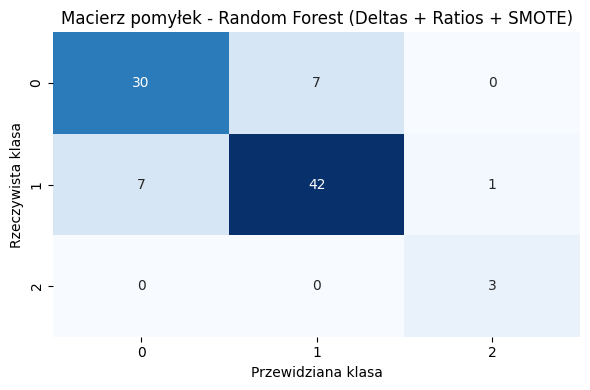
\includegraphics[width=0.7\textwidth]{rf_eng.png}
    \caption{Macierz pomyłek dla modelu Random Forest z inżynierią cech.}
    \label{fig:rf_eng}
\end{figure}

Jest to najlepszy z dotychczasowych wariantów algorytmu Random Forest w kontekście detekcji klasy mniejszościowej. Uzyskanie czułości (\textit{Recall}) na poziomie $1,00$ oznacza bezbłędne rozpoznanie wszystkich patologicznych przypadków \textit{vertical}, pomimo że stanowią one zaledwie 16 obserwacji w całym zbiorze.






\subsection{K-Nearest Neighbors}

\subsubsection{Bazowy algorytm K-Nearest Neighbors}

W pierwszym kroku ewaluacji poddano bazowy wariant algorytmu K-Najbliższych Sąsiadów (KNN). Z uwagi na fakt, że KNN opiera swoje działanie na miarach odległości pomiędzy punktami, kluczowym elementem potoku przetwarzania (\textit{pipeline}) była standaryzacja danych za pomocą \texttt{StandardScaler}.
W procesie kroswalidacji model uzyskał średni wynik F1-macro na poziomie $0{,}5003 \pm 0{,}0673$. 

Szczegółowe wyniki klasyfikacji na zbiorze testowym przedstawiono w Tabeli \ref{tab:knn_baseline_results}.

\begin{table}[H]
\centering
\caption{Metryki klasyfikacji dla bazowego modelu KNN}
\label{tab:knn_baseline_results}
\begin{tabular}{@{}lcccc@{}}
\toprule
\textbf{Klasa} & \textbf{Precision} & \textbf{Recall} & \textbf{F1-score} & \textbf{Support} \\ \midrule
0              & 0,80               & 0,76            & 0,78              & 37               \\
1              & 0,78               & 0,86            & 0,82              & 50               \\
2              & 0,00               & 0,00            & 0,00              & 3                \\ \midrule
\textbf{Accuracy}       & \multicolumn{2}{c}{---}       & \textbf{0,79}     & 90               \\
\textbf{Macro avg}      & 0,53               & 0,54            & 0,53              & 90               \\
\textbf{Weighted avg}   & 0,76               & 0,79            & 0,77              & 90               \\ \bottomrule
\end{tabular}
\end{table}

\begin{figure}[H]
    \centering
    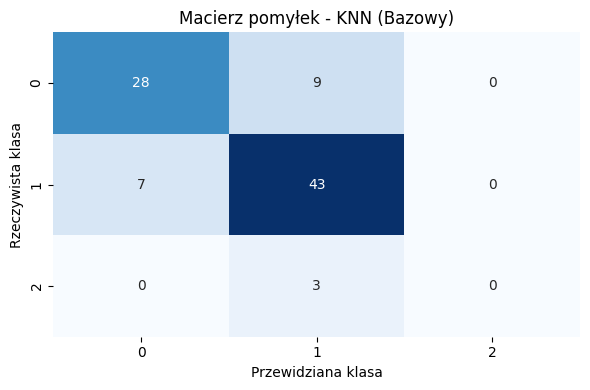
\includegraphics[width=0.7\textwidth]{knn_base.png} % Upewnij się, że masz ten plik
    \caption{Macierz pomyłek dla bazowego modelu KNN}
    \label{fig:knn_base}
\end{figure}

Podobnie jak w przypadku bazowych wersji Drzewa Decyzyjnego i Lasu Losowego, podstawowy algorytm KNN wykazuje całkowitą niezdolność do detekcji klasy 2 (\textit{vertical}). Przypisywanie obserwacji wyłącznie do klas większościowych zaowocowało ostrzeżeniem środowiska o zerowej precyzji (\textit{UndefinedMetricWarning}), co jednoznacznie potwierdza konieczność zastosowania technik balansowania danych.

\subsubsection{K-Nearest Neighbors z techniką SMOTE}

Aby rozwiązać problem niedoreprezentowanej klasy, do potoku przetwarzania (pomiędzy skaler a klasyfikator) wprowadzono algorytm \textit{oversamplingu} SMOTE. 
W procesie kroswalidacji średni wynik F1-macro modelu wzrósł do $0{,}5537 \pm 0{,}0861$.

\begin{table}[H]
\centering
\caption{Metryki klasyfikacji dla modelu KNN z techniką SMOTE}
\label{tab:knn_smote_results}
\begin{tabular}{@{}lcccc@{}}
\toprule
\textbf{Klasa} & \textbf{Precision} & \textbf{Recall} & \textbf{F1-score} & \textbf{Support} \\ \midrule
0              & 0,72               & 0,84            & 0,78              & 37               \\
1              & 0,88               & 0,72            & 0,79              & 50               \\
2              & 0,50               & 1,00            & 0,67              & 3                \\ \midrule
\textbf{Accuracy}       & \multicolumn{2}{c}{---}       & \textbf{0,78}     & 90               \\
\textbf{Macro avg}      & 0,70               & 0,85            & 0,74              & 90               \\
\textbf{Weighted avg}   & 0,80               & 0,78            & 0,78              & 90               \\ \bottomrule
\end{tabular}
\end{table}

\begin{figure}[H]
    \centering
    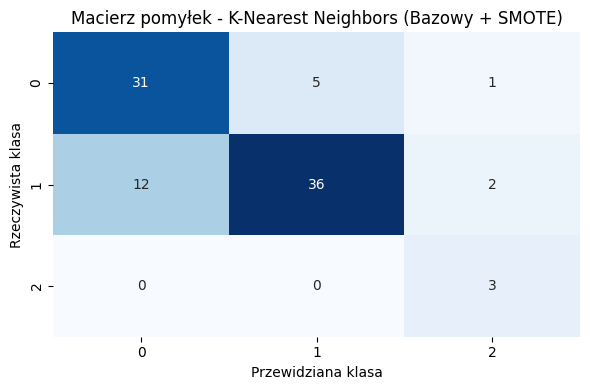
\includegraphics[width=0.7\textwidth]{knn_smote.png} % Upewnij się, że masz ten plik
    \caption{Macierz pomyłek dla modelu KNN z techniką SMOTE}
    \label{fig:knn_smote}
\end{figure}

Zastosowanie SMOTE przyniosło radykalną poprawę. Czułość (\textit{Recall}) dla klasy 2 osiągnęła poziom 1,00, co oznacza bezbłędne zidentyfikowanie wszystkich przypadków patologicznych ze zbioru testowego. Mimo iż precyzja dla tej klasy wynosi 0,50 (pojawiają się fałszywe alarmy), to ogólna miara F1-macro wzrosła z 0,53 do 0,74 przy jedynie marginalnym spadku ogólnej trafności (\textit{Accuracy} = 0,78 względem 0,79).

\subsubsection{Optymalizacja K-Nearest Neighbors (Grid Search + SMOTE)}

W kolejnym kroku przeprowadzono optymalizację hiperparametrów za pomocą \textit{Grid Search}. Przeszukiwano m.in. liczbę sąsiadów, metryki odległości (parametr $p$) oraz typ wag. Optymalny model charakteryzował się następującymi parametrami:
\begin{itemize}
    \item \textbf{n\_neighbors:} 9,
    \item \textbf{metric:} minkowski,
    \item \textbf{p:} 2 (odległość euklidesowa),
    \item \textbf{weights:} uniform.
\end{itemize}

Średni wynik kroswalidacji uległ poprawie, osiągając F1-macro równe $0{,}5773 \pm 0{,}0699$.

\begin{table}[H]
\centering
\caption{Metryki klasyfikacji dla zoptymalizowanego modelu KNN (Grid Search + SMOTE)}
\label{tab:knn_opt_results}
\begin{tabular}{@{}lcccc@{}}
\toprule
\textbf{Klasa} & \textbf{Precision} & \textbf{Recall} & \textbf{F1-score} & \textbf{Support} \\ \midrule
0              & 0,71               & 0,86            & 0,78              & 37               \\
1              & 0,89               & 0,68            & 0,77              & 50               \\
2              & 0,43               & 1,00            & 0,60              & 3                \\ \midrule
\textbf{Accuracy}       & \multicolumn{2}{c}{---}       & \textbf{0,77}     & 90               \\
\textbf{Macro avg}      & 0,68               & 0,85            & 0,72              & 90               \\
\textbf{Weighted avg}   & 0,80               & 0,77            & 0,77              & 90               \\ \bottomrule
\end{tabular}
\end{table}

\begin{figure}[H]
    \centering
    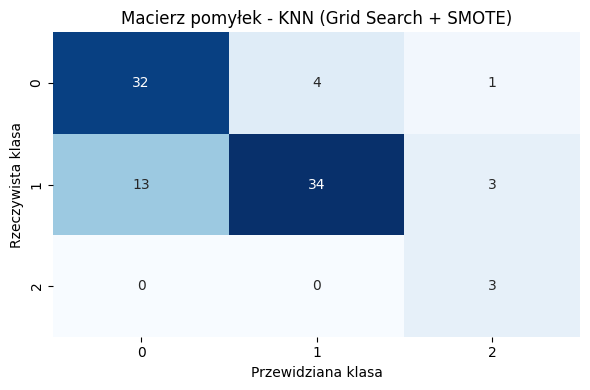
\includegraphics[width=0.7\textwidth]{knn_opt.png} % Upewnij się, że masz ten plik
    \caption{Macierz pomyłek dla zoptymalizowanego modelu KNN}
    \label{fig:knn_opt}
\end{figure}

Zwiększenie liczby rozpatrywanych sąsiadów do 9 pozwoliło modelowi uogólniać wiedzę lepiej (wyższy wynik kroswalidacji), choć nie przełożyło się to na drastyczny wzrost metryk na zbiorze testowym w stosunku do wariantu domyślnego. Model utrzymał maksymalną czułość dla rzadkiej klasy 2.

\subsubsection{Zaawansowana inżynieria cech (Deltas + PCA + SMOTE + GridSearch)}

W ostatnim eksperymencie z algorytmem KNN zastosowano złożony potok przetwarzania. Wzorując się na poprzednich algorytmach, obliczono zmienne różnicowe (\textit{Deltas}). Z uwagi na podatność KNN na zjawisko „klątwy wymiarowości” oraz wysoki poziom korelacji cech, wprowadzono redukcję wymiarowości za pomocą Analizy Głównych Składowych (PCA), zachowując 95\% wariancji.

Wynik \textit{Grid Search} wyłonił optymalne parametry (\texttt{n\_neighbors: 3, p: 2, weights: uniform}), a model uzyskał wynik CV na poziomie $0{,}5387 \pm 0{,}0614$. Ewaluacja na zbiorze testowym ujawniła jednak poważne problemy tego podejścia (Tabela \ref{tab:knn_adv_results}).

\begin{table}[H]
\centering
\caption{Metryki dla modelu KNN z inżynierią cech i PCA}
\label{tab:knn_adv_results}
\begin{tabular}{@{}lcccc@{}}
\toprule
\textbf{Klasa} & \textbf{Precision} & \textbf{Recall} & \textbf{F1-score} & \textbf{Support} \\ \midrule
0              & 0,49               & 0,62            & 0,55              & 37               \\
1              & 0,66               & 0,46            & 0,54              & 50               \\
2              & 0,38               & 1,00            & 0,55              & 3                \\ \midrule
\textbf{Accuracy}       & \multicolumn{2}{c}{---}       & \textbf{0,54}     & 90               \\
\textbf{Macro avg}      & 0,51               & 0,69            & 0,54              & 90               \\
\textbf{Weighted avg}   & 0,58               & 0,54            & 0,54              & 90               \\ \bottomrule
\end{tabular}
\end{table}

\begin{figure}[H]
    \centering
    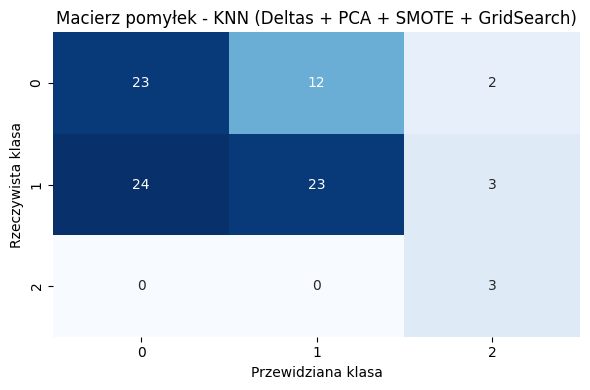
\includegraphics[width=0.7\textwidth]{knn_adv.png} % Upewnij się, że masz ten plik
    \caption{Macierz pomyłek dla modelu KNN z zaawansowaną inżynierią cech}
    \label{fig:knn_adv}
\end{figure}

W przeciwieństwie do modelu Random Forest, transformacja cech w połączeniu z redukcją przestrzeni (PCA) doprowadziła do drastycznego spadku ogólnej trafności klasyfikatora (\textit{Accuracy} na poziomie 0,54). Chociaż model wciąż doskonale wykrywa klasę 2 (\textit{Recall} równe 1,00), całkowicie zatracił zdolność precyzyjnego rozróżniania klas 0 i 1. Dowodzi to, że transformacja przestrzeni cech poprzez PCA zaburzyła oryginalne metryki odległości, na których opiera się KNN, prowadząc do znacznej utraty skuteczności na klasach większościowych. W przypadku tego zbioru danych, algorytmy oparte na zespołach drzew (Random Forest) radzą sobie ze skomplikowaną inżynierią cech znacznie lepiej niż algorytmy oparte na odległości.

\subsection{Wnioski końcowe}
Na podstawie uzyskanych wyników można sformułować następujące wnioski:
\begin{itemize}
    \item \textbf{Zespoły drzew decyzyjnych dominują:} Algorytm Random Forest okazał się najbardziej stabilnym i skutecznym modelem. Jego zoptymalizowana wersja z inżynierią cech osiągnęła imponującą czułość (\textit{Recall} = 1,00) dla klasy mniejszościowej przy zachowaniu wysokiej ogólnej dokładności (\textit{Accuracy} = 0,83).
     \item \textbf{Wpływ inżynierii cech:} Zastosowanie zaawansowanych przekształceń danych, takich jak tworzenie zmiennych różnicowych (Deltas) oraz wskaźników proporcji (Ratios), w połączeniu z redukcją współliniowości, przyniosło zróżnicowane efekty w zależności od specyfiki algorytmu. W modelach opartych na zespołach drzew (Random Forest) oraz pojedynczych drzewach decyzyjnych, inżynieria cech okazała się pomocna dla osiągnięcia bezbłędnej detekcji patologicznych przypadków z mniejszościowej klasy 2. Z kolei w przypadku algorytmów opartych na odległości, takich jak K-Nearest Neighbors, transformacja przestrzeni cech połączona z redukcją wymiarowości (PCA) drastycznie zaburzyła oryginalne metryki odległości, co doprowadziło do znacznej utraty skuteczności klasyfikatora na klasach większościowych i spadku ogólnej trafności modelu.
    \item \textbf{Ostrożność przy oversamplingu:} Zastosowanie techniki SMOTE było niezbędne do wykrycia klasy mniejszościowej, jednak bez odpowiedniej regularyzacji hiperparametrów (np. drastycznego ograniczenia głębokości drzewa) prowadziło to do silnego przeuczenia modelu na syntetycznym szumie.
\item \textbf{Ograniczenia algorytmów opartych na odległości:} Algorytm K-Nearest Neighbors okazał się najmniej przystosowany do natury tego zbioru danych. Próba zaawansowanej redukcji wymiarowości (PCA) w celu zniwelowania współliniowości całkowicie zaburzyła metryki odległości, drastycznie pogarszając zdolności klasyfikacyjne modelu. Algorytm PCA opiera się na maksymalizacji wariancji, co w przypadku tak silnie niezrównoważonych danych oznacza, że subtelne różnice definiujące klasę mniejszościową (\textit{vertical}) mogły zostać potraktowane jako szum i odrzucone w procesie redukcji (przy zachowaniu 95\% wariancji). To sprawiło, że model KNN całkowicie „oślepł” na te rzadkie, lokalne klastry.
\end{itemize}

Ostatecznie, modelem rekomendowanym do ewentualnego wdrożenia wspomagającego diagnozę lub do dalszych testów jest zoptymalizowany Random Forest połączony z inżynierią cech i algorytmem SMOTE.

\subsection{Propozycje dalszych badań}
Z uwagi na specyfikę biomedycznych danych analitycznych oraz napotkane wyzwania, proponuje się następujące kierunki dalszych prac rozwojowych:
\begin{itemize}
    \item \textbf{Rozszerzenie zbioru danych:} Najbardziej naturalnym i pożądanym krokiem jest pozyskanie większej liczby danych pacjentów z patologicznym kierunkiem wzrostu (\textit{vertical}). Zwiększenie rzeczywistej reprezentacji tej klasy pozwoliłoby na weryfikację modeli bez konieczności polegania na sztucznym oversamplingu.
    \item \textbf{Testowanie algorytmów Gradient Boosting:} Warto sprawdzić skuteczność nowoczesnych algorytmów wzmacniania gradientowego (np. XGBoost), które natywnie świetnie radzą sobie z danymi tabelarycznymi i oferują wbudowane, zoptymalizowane mechanizmy obsługi niezrównoważonych klas.
    \item \textbf{Uczenie wrażliwe na koszty (Cost-sensitive learning):} Zamiast generować syntetyczne próbki (SMOTE), alternatywnym podejściem jest modyfikacja funkcji kosztu algorytmów tak, aby błąd w klasyfikacji rzadkiej klasy 2 był karany znacznie surowiej niż pomyłki w klasach większościowych.
    \item \textbf{Zaawansowane techniki resamplingu:} Eksploracja zaawansowanych metod balansowania danych. Metody te oprócz generowania nowych próbek, usuwają również szum i obserwacje z pogranicza klas, co mogłoby poprawić precyzję (zmniejszyć liczbę fałszywych alarmów dla rzadkich diagnoz).
\end{itemize}







\section{Regresja}
\subsection{Streszczenie i krótki opis danych}

W części regresyjnej rozwiązujemy problem \textbf{predykcji ceny sprzedaży domu} (\texttt{SalePrice}) na podstawie cech opisujących nieruchomość ze zbioru \textit{Ames Housing}. 

W ramach analizy porównano kilka podejść: model liniowy bazowy, warianty po selekcji cech, model z transformacją celu \texttt{log1p(SalePrice)}, modele drzewiaste (Random Forest i XGBoost) oraz ensembling. Najlepszy pojedynczy model stanowił Random Forest, natomiast \textbf{najlepszy wynik końcowy} uzyskał model zespołowy (weighted ensemble), który osiągnął najniższy błąd RMSE i najwyższe $R^2$ na zbiorze testowym.
\subsection{Analiza i preprocessing danych}

\subsubsection{Wstępna analiza danych}

Na początku części regresyjnej wykonano eksploracyjną analizę danych (EDA), aby scharakteryzować rozkład zmiennej celu \texttt{SalePrice}. Podstawowe statystyki opisowe cen domów były następujące:
\begin{table}[H]
\centering
\begin{tabular}{|l|r|}
\hline
\textbf{Statystyka} & \textbf{Wartość} \\ \hline
Liczba obserwacji & 1456 \\ \hline
Wartość średnia & 180\,151.23 \\ \hline
Odchylenie standardowe & 76\,696.59 \\ \hline
Wartość minimalna & 34\,900 \\ \hline
Kwartyl 1 (25\%) & 129\,900 \\ \hline
Mediana (50\%) & 163\,000 \\ \hline
Kwartyl 3 (75\%) & 214\,000 \\ \hline
Wartość maksymalna & 625\,000 \\ \hline
\end{tabular}
\caption{Podstawowe statystyki opisowe zmiennej \texttt{SalePrice}}
\label{tab:saleprice-stats}
\end{table}

Jak można wywnioskować z danych statystycznych większość domów w zbiorze to nieruchomości tańsze i o średniej cenie. Koncentracja rynku (Interquartile Range): Połowa badanych nieruchomości (zakres między 1. a 3. kwartylem) mieści się w przedziale cenowym od 129900 do 214000. Można zatem uznać ten zakres za "typowy" dla analizowanego segmentu rynku.

Dodatkowo przeanalizowano zależności pomiędzy zmiennymi numerycznymi za pomocą mapy cieplnej korelacji (Rysunek \ref{fig:reg-correlation-heatmap}), co pozwoliło zidentyfikować grupy silnie skorelowanych cech i uzasadniło późniejszy eksperyment z usuwaniem kolumn o wysokiej współliniowości.

\begin{figure}[H]
    \centering
    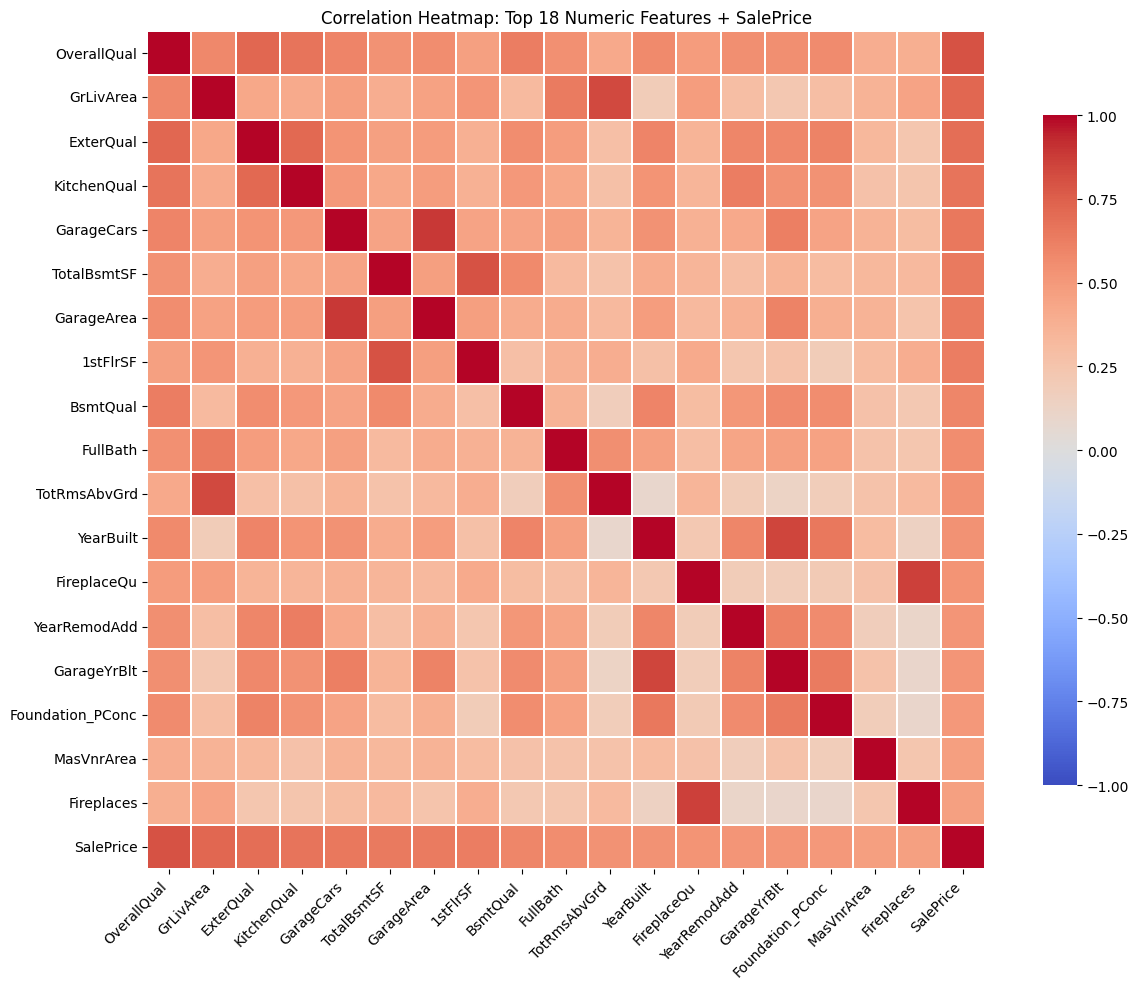
\includegraphics[width=0.95\textwidth]{corellation_heatmap_reg.png}
    \caption{Mapa cieplna korelacji cech w zadaniu regresji}
    \label{fig:reg-correlation-heatmap}
\end{figure}

\subsubsection{Preprocessing danych}

W zadaniu regresji wykorzystano zbiór \textit{Ames Housing}, w którym zmienną celu była cena sprzedaży domu (\texttt{SalePrice}). Po wstępnym czyszczeniu usunięto obserwacje odstające dla bardzo dużych powierzchni użytkowych (\texttt{GrLivArea} $>$ 4000), co ograniczyło wpływ skrajnych punktów na model liniowy. Następnie przeprowadzono imputację braków danych zgodnie z charakterem cech (wartość \texttt{None}, zero lub imputacja medianą/modą), a dla cech kategorycznych zastosowano kodowanie porządkowe i \textit{one-hot encoding}.



Po przygotowaniu danych zdefiniowano macierz cech \texttt{X} i zmienną celu \texttt{y}, a następnie wykonano podział na zbiory treningowy i testowy (80/20). Dla modeli liniowych zastosowano standaryzację przy użyciu \texttt{StandardScaler} dopasowanego wyłącznie na zbiorze treningowym, aby uniknąć wycieku informacji.


\subsection{Model bazowy: regresja liniowa}

Jako punkt odniesienia przyjęto klasyczną regresję liniową. Ocenę modelu przeprowadzono dwuetapowo:
\begin{itemize}
    \item walidacja krzyżowa 5-fold na zbiorze treningowym,
    \item finalna ewaluacja na wydzielonym zbiorze testowym.
\end{itemize}


\subsubsection{Eksperyment 1: usuwanie prawie stałych kolumn}

W pierwszym eksperymencie usunięto kolumny prawie stałe (próg dominacji jednej wartości: 97\%). Celem było ograniczenie szumu i usunięcie cech o niskiej wartości informacyjnej dla modelu liniowego.

Wyniki metryk dla modelu bazowego i obu eksperymentów zestawiono w Tabeli \ref{tab:linear_feature_experiments}.

Interpretacja: metryki walidacji krzyżowej wyraźnie się poprawiły, natomiast wynik na zbiorze testowym pozostał bardzo zbliżony do bazowego (lekko gorszy dla RMSE i $R^2$). Oznacza to, że redukcja cech prawie stałych może stabilizować uczenie, ale w tym przypadku nie przełożyła się na jednoznaczny zysk generalizacji.

\subsubsection{Eksperyment 2: usuwanie silnie skorelowanych kolumn}

W drugim eksperymencie usunięto jedną cechę z każdej pary silnie skorelowanej (próg $|r| > 0.9$). Łącznie odrzucono 13 kolumn, redukując przestrzeń cech z 230 do 217 wymiarów.

\begin{table}[H]
\centering
\caption{Regresja liniowa: porównanie metryk modelu bazowego i eksperymentów selekcji cech}
\label{tab:linear_feature_experiments}
\begin{tabular}{|l|c|c|c|c|c|c|}
\hline
\textbf{Wariant} & \textbf{CV RMSE} & \textbf{CV MAE} & \textbf{CV $R^2$} & \textbf{Test RMSE} & \textbf{Test MAE} & \textbf{Test $R^2$} \\
\hline
Model bazowy & 28\,027.33 $\pm$ 2\,266.96 & 19\,124.67 $\pm$ 1\,039.61 & 0.8656 $\pm$ 0.0265 & 23\,471.16 & 17\,339.86 & 0.8950 \\
Bez near-constant & 26\,335.93 $\pm$ 2\,568.77 & 18\,049.59 $\pm$ 669.41 & 0.8833 $\pm$ 0.0117 & 23\,588.46 & 17\,472.24 & 0.8940 \\
Bez silnie skorelowanych & 27\,922.86 $\pm$ 2\,263.75 & 19\,139.69 $\pm$ 976.08 & 0.8667 $\pm$ 0.0256 & 23\,589.82 & 17\,280.95 & 0.8940 \\
\hline
\end{tabular}
\end{table}

Interpretacja: wyniki są praktycznie równoważne modelowi bazowemu. Usunięcie części kolumn skorelowanych uprościło model, ale nie poprawiło jakości predykcji w sposób istotny. Z tego eksperymentu wnioskuję, że warto zainteresować się upraszczaniem modelu (w przypadku większej liczby danych i/lub cech) aby ograniczyć czas i zasoby potrzebne do wytrenowania modelu, ponieważ może się okazać (jak w tym przypadku) że można zredukować liczbę cech i nie utracić przy tym znacząco jakości modelu.

\subsubsection{Eksperyment 3: feature engineering}

W aktualnej wersji eksperymentu rozszerzono zbiór o \textbf{4} ręcznie zaprojektowane cechy: \texttt{HouseAge}, \texttt{RemodAge}, \texttt{HasGarage} oraz \texttt{HasBasement}. Celem było sprawdzenie, czy proste cechy opisujące wiek budynku i obecność kluczowych elementów infrastruktury poprawią jakość modelu liniowego.

Porównanie z modelem bazowym pokazuje, że wpływ tego wariantu był \textbf{niewielki}:
\begin{itemize}
    \item \textbf{Test RMSE:} 23\,471.16 $\rightarrow$ 23\,448.24,
    \item \textbf{Test MAE:} 17\,339.86 $\rightarrow$ 17\,327.24,
    \item \textbf{Test $R^2$:} 0.8950 $\rightarrow$ 0.8952.
\end{itemize}

Również metryki walidacji krzyżowej pozostały praktycznie bez zmian (CV RMSE 28\,026.68 $\pm$ 2\,266.43), co potwierdza, że ten zestaw cech dodał ograniczoną wartość predykcyjną.

\subsubsection{Eksperyment4: transformacja zmiennej celu \texttt{log1p(SalePrice)}}
\begin{figure}[H]
    \centering
    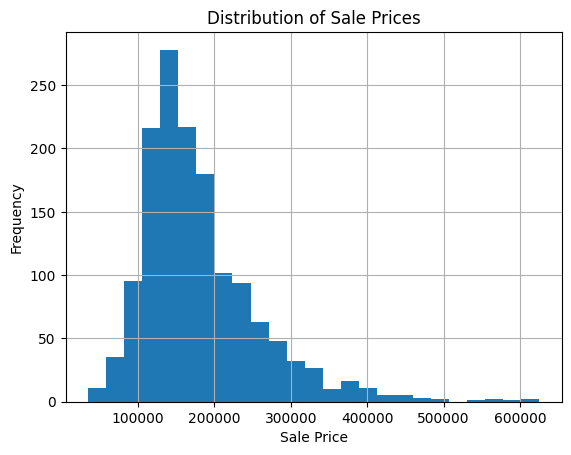
\includegraphics[width=0.78\textwidth]{output_rozklad.png}
    \caption{Rozkład cen}
    \label{fig:output_rozklad}
\end{figure}
W celu ograniczenia wpływu prawostronnej skośności cen nieruchomości oraz poprawy stabilności błędu przetestowano wariant regresji liniowej z transformacją zmiennej celu: $y_{log}=\log(1+\texttt{SalePrice})$. Model trenowano na przekształconym celu, a predykcje na etapie ewaluacji odwracano funkcją $\exp(\hat{y}_{log})-1$.

Eksperyment wykazał wyraźną poprawę jakości predykcji na zbiorze testowym. RMSE spadło z \textbf{23\,471.16} (model bazowy) do \textbf{20\,732.78}, co oznacza poprawę o około \textbf{11.7\%}. Jednocześnie poprawiły się także pozostałe metryki: MAE zmalało z 17\,339.86 do 14\,742.18, a współczynnik $R^2$ wzrósł z 0.8950 do 0.9181. Wynik ten wskazuje, że transformacja targetu była jednym z najbardziej efektywnych usprawnień dla modelu liniowego w całej analizie regresyjnej.

\begin{table}[H]
\centering
\caption{Porównanie regresji liniowej: \texttt{SalePrice} vs \texttt{log1p(SalePrice)}}
\label{tab:log_target_compare}
\begin{tabular}{|l|c|c|c|}
\hline
\textbf{Model} & \textbf{RMSE} & \textbf{MAE} & \textbf{$R^2$} \\
\hline
Linear (SalePrice) & 23\,471.16 & 17\,339.86 & 0.8950 \\
Linear (log1p SalePrice) & 20\,732.78 & 14\,742.18 & 0.9181 \\
\hline
\end{tabular}
\end{table}


\subsection{Dodatkowo przetestowane modele: Random Forest i XGBoost}

Poza regresją liniową przetestowano również dwa modele nieliniowe: \texttt{RandomForestRegressor} oraz \texttt{XGBRegressor}. Celem było sprawdzenie, czy modele drzewiaste, lepiej opisujące zależności nieliniowe i interakcje cech, poprawią jakość predykcji względem podejścia liniowego.

\subsubsection*{Porównanie walidacji krzyżowej (5-fold)}

\begin{table}[H]
\centering
\caption{Porównanie modeli na walidacji krzyżowej (zbiór treningowy)}
\label{tab:regression_cv_compare}
\begin{tabular}{|l|c|c|c|}
\hline
\textbf{Model} & \textbf{CV RMSE} & \textbf{CV MAE} & \textbf{CV $R^2$} \\
\hline
Linear Regression (bazowy) & 28\,027.33 $\pm$ 2\,266.96 & 19\,124.67 $\pm$ 1\,039.61 & 0.8656 \\
Linear Regression (bez near-constant) & 26\,335.93 $\pm$ 2\,568.77 & 18\,049.59 $\pm$ 669.41 & 0.8833 \\
Linear Regression (bez silnie skorelowanych) & 27\,922.86 $\pm$ 2\,263.75 & 19\,139.69 $\pm$ 976.08 & 0.8667  \\
Random Forest & 26\,930.54 $\pm$ 3\,680.44 & 17\,037.75 $\pm$ 1\,997.39 & 0.8785  \\
XGBoost & 27\,307.76 $\pm$ 2\,622.92 & 17\,737.87 $\pm$ 1\,218.76 & 0.8753 \\
\hline
\end{tabular}
\end{table}

\subsubsection*{Porównanie wyników na zbiorze testowym}

\begin{table}[H]
\centering
\caption{Porównanie modeli na zbiorze testowym}
\label{tab:regression_test_compare}
\begin{tabular}{|l|c|c|c|}
\hline
\textbf{Model} & \textbf{Test RMSE} & \textbf{Test MAE} & \textbf{Test $R^2$} \\
\hline
Linear Regression (bazowy) & 23\,471.16 & 17\,339.86 & 0.8950 \\
Linear Regression (bez near-constant) & 23\,588.46 & 17\,472.24 & 0.8940 \\
Linear Regression (bez silnie skorelowanych) & 23\,589.82 & 17\,280.95 & 0.8940 \\
Random Forest & 22\,961.69 & 16\,337.33 & 0.8995 \\
XGBoost & 24\,866.80 & 16\,888.02 & 0.8822 \\
\hline
\end{tabular}
\end{table}

\subsubsection*{Wpływ transformacji \texttt{log1p(SalePrice)} na Random Forest}

Ponieważ transformacja targetu \texttt{log1p(SalePrice)} wyraźnie poprawiła regresję liniową, przetestowano ten sam zabieg dla modelu \texttt{RandomForestRegressor}. Porównanie wykonano rzetelnie na tych samych foldach walidacji krzyżowej (5-fold), a następnie potwierdzono na zbiorze testowym.

Wynik był odwrotny niż dla modelu liniowego: transformacja \texttt{log1p} pogorszyła metryki.
\begin{table}[H]
\centering
\caption{Random Forest: porównanie wariantu bazowego i wariantu z \texttt{log1p(SalePrice)}}
\label{tab:rf_log_target_compare}
\begin{tabular}{|l|c|c|}
\hline
\textbf{Metryka} & \textbf{RF bazowy} & \textbf{RF z \texttt{log1p} targetu} \\
\hline
CV RMSE & 26\,930.54 $\pm$ 3\,680.44 & 27\,730.40 $\pm$ 4\,081.41 \\
CV MAE & 17\,037.75 $\pm$ 1\,997.39 & 17\,408.87 $\pm$ 2\,365.24 \\
CV $R^2$ & 0.8785 $\pm$ 0.0223 & 0.8716 $\pm$ 0.0241 \\
Test RMSE & 22\,961.69 & 24\,917.28 \\
Test MAE & 16\,337.33 & 16\,845.53 \\
Test $R^2$ & 0.8995 & 0.8817 \\
\hline
\end{tabular}
\end{table}

Interpretacja: modele drzewiaste (w tym Random Forest) dobrze modelują nieliniowości i skrajne zakresy wartości bez transformacji celu. Dodatkowa kompresja skali przez logarytm może osłabiać informację o wysokich cenach, co w tym przypadku przełożyło się na gorszą jakość predykcji.

\begin{figure}[H]
    \centering
    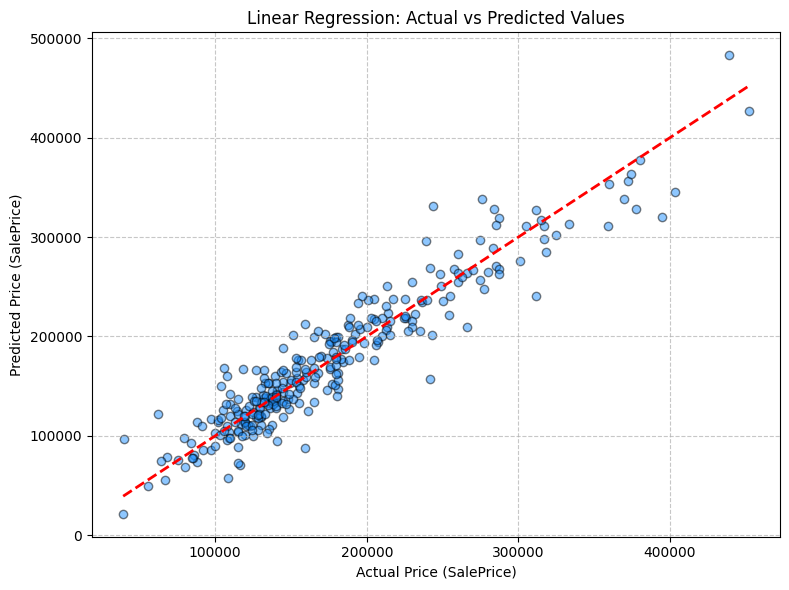
\includegraphics[width=0.78\textwidth]{reg_linear_actual_vs_pred.png}
    \caption{Regresja liniowa: wartości rzeczywiste vs przewidywane na zbiorze testowym}
    \label{fig:reg_linear_actual_pred}
\end{figure}



Wyniki pokazują, że \textbf{Random Forest} osiągnął najlepszy wynik na zbiorze testowym (najniższy RMSE i najwyższe $R^2$), natomiast \textbf{XGBoost} w obecnej konfiguracji nie poprawił jakości względem modelu bazowego.

\subsection{Ensembling modeli (kod wygenerowano w pełni przy wykorzsytaniu LLM)}

W ostatnim etapie sprawdzono prosty ensembling oparty na średniej ważonej predykcji trzech modeli: regresji liniowej, regresji liniowej z transformacją \texttt{log1p(SalePrice)} oraz Random Forest. Wagi dobrano na zbiorze walidacyjnym; najlepszy wariant uzyskał konfigurację: \texttt{LR=0.00}, \texttt{LR\_log=0.60}, \texttt{RF=0.40}.

\begin{table}[H]
\centering
\caption{Porównanie modeli i ensemblingu na zbiorze testowym}
\label{tab:ensemble_test_compare}
\begin{tabular}{|l|c|}
\hline
\textbf{Model} & \textbf{Test RMSE} \\
\hline
Weighted Ensemble (LR=0.00, LR\_log=0.60, RF=0.40) & 20\,006.23 \\
Linear Regression (log1p target) & 22\,434.93 \\
Random Forest & 23\,637.55 \\
Linear Regression & 25\,846.25 \\
\hline
\end{tabular}
\end{table}

\begin{figure}[H]
    \centering
    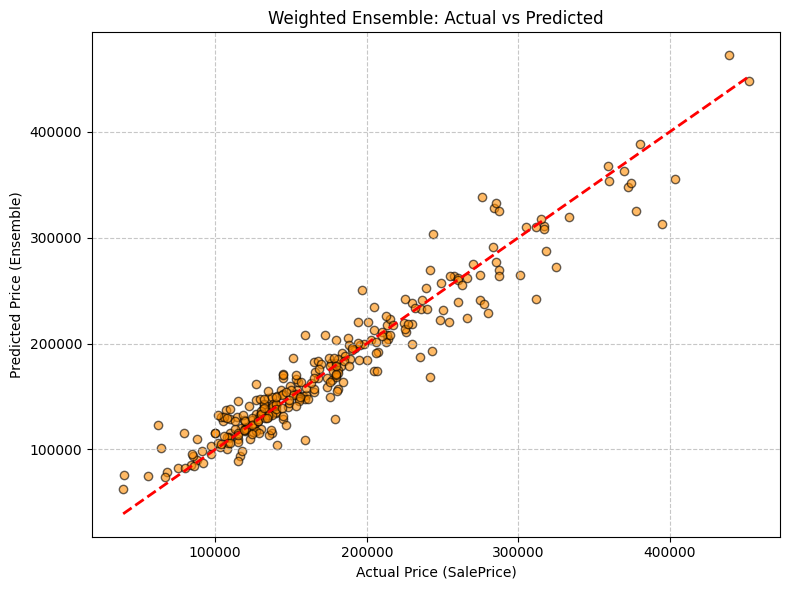
\includegraphics[width=0.78\textwidth]{ensembl1.png}
    \caption{Ensmebling modeli: wartości rzeczywiste vs przewidywane na zbiorze testowym}
    \label{fig:ensembl1}
\end{figure}

\begin{figure}[H]
    \centering
    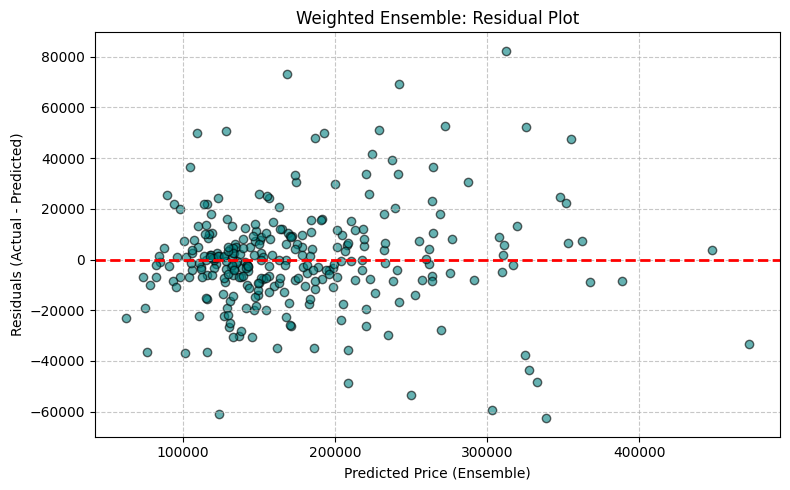
\includegraphics[width=0.78\textwidth]{ensemble2_residual.png}
    \caption{Ensmebling modeli: Residual}
    \label{fig:ensembl1}
\end{figure}


Dla najlepszego ensemblingu na zbiorze testowym uzyskano: \textbf{RMSE = 20\,006.23}, \textbf{MAE = 13\,749.34} oraz \textbf{$R^2 = 0.9237$}. Krótko: ensembling dał najlepszy wynik końcowy i wyraźnie poprawił jakość względem pojedynczych modeli.

\subsection{Wnioski końcowe dla regresji}

\begin{itemize}
    \item Wykonane eksperymenty selekcji cech były \textbf{wartościowe diagnostycznie}: pokazały, że część redukcji wymiarowości może uprościć model bez dużej utraty jakości.
    \item Największa poprawa pojawiła się w metrykach CV po usunięciu cech prawie stałych, jednak \textbf{na zbiorze testowym zysk nie został potwierdzony}.
    \item Usuwanie cech silnie skorelowanych dało \textbf{minimalny wpływ} na metryki końcowe, co sugeruje, że przy aktualnym pipeline model bazowy już dobrze wykorzystuje informację z danych.
    \item W dodatkowym wariancie redukcji wymiarowości usunięcie ok. 107 z 250 kolumn (ok. 43\%) nie pogarszało istotnie jakości modelu. Taka redukcja liczby cech jest szczególnie cenna praktycznie, ponieważ przy większej liczbie rekordów i większym wymiarze danych znacząco skracałaby czas trenowania oraz koszt obliczeniowy.
    \item Transformacja targetu \texttt{log1p(SalePrice)} poprawiła regresję liniową, ale \textbf{pogorszyła} wyniki Random Forest zarówno w CV, jak i na zbiorze testowym.
    \item Rozszerzenie analizy o \textbf{Random Forest i XGBoost} było zasadne: Random Forest okazał się najlepszym pojedynczym modelem końcowym, a XGBoost wskazał potrzebę dalszego strojenia hiperparametrów.
    \item Ciekawym eksperymentem był ensembling modeli, który doprowadził do uzyskania najlepszego wyniku.
\end{itemize}

\subsection{Potencjalne dalsze eksperymenty}

W przyszłości warto byłoby popracować nad:
\begin{itemize}
    \item \textbf{Głębszy feature engineering:} dodanie kolejnych cech opartych na wiedzy dziedzinowej, np. interakcji między cechami, cech ilorazowych/różnicowych oraz cech agregujących informacje o standardzie i wielkości nieruchomości.
    \item \textbf{Systematyczne strojenie hiperparametrów:} zastosowanie \texttt{RandomizedSearchCV} lub \texttt{GridSearchCV} dla modeli liniowych i drzewiastych (szczególnie \texttt{XGBoost}).
   
    \item \textbf{Eksperymenty z walidacją:} wykorzystanie walidacji powtarzanej (\textit{Repeated K-Fold}) oraz porównanie stabilności metryk między różnymi losowaniami podziału danych.
    \item \textbf{Analiza błędów predykcji:} osobna diagnostyka przypadków z największym błędem (np. najdroższe domy), aby zidentyfikować brakujące informacje i kierunki dalszego feature engineeringu.
\end{itemize}


\section{Podział prac między członkami grupy}
W ramach projektu zadania zostały rozdzielone w następujący sposób:

\begin{itemize}
    \item \textbf{Mateusz Stawicki} - odpowiedzialny za realizację większości zadań związanych z regresją.
    \item \textbf{Maciej Kondratowicz} - odpowiedzialny za większość zadań związanych z klasyfikacją.
\end{itemize}

\section{Wykorzystanie sztucznej inteligencji}
W procesie tworzenia projektu szeroko wykorzystywano modele typu LLM (Large Language Models). Narzędzia te służyły do:
\begin{itemize}
    \item wsparcia podczas pisania raportu i dokumentacji,
    \item generowania fragmentów kodu,
    \item pomaganiu przy przeprowadzaniu researchu
\end{itemize}

Fragmenty tekstu oraz kodu wygenerowane przez AI został poddane weryfikacji oraz poprawieniu przez członków zespołu.

\end{document}